\documentclass{article}
\usepackage[polish]{babel}
\usepackage[utf8]{inputenc}
\usepackage[T1]{fontenc}
\usepackage{graphicx}
\usepackage{array}
\newcolumntype{L}{>{\centering\arraybackslash}m{7cm}}
\usepackage{enumitem}

\usepackage{fancyhdr}
\usepackage{lastpage}

\pagestyle{fancy}
\fancyhf{}

\rfoot{Strona \thepage \hspace{1pt} z \pageref{LastPage}}


\title{Specyfikacja funkcjonalna projektu zespołowego "Symulator przewożenia pacjentów do szpitali w Polsce"}
\author{Michał Wójcik, Marek Nowakowski, Filip Olejniczak}
\date{18 listopada 2020}

\begin{document}

\maketitle

\tableofcontents
\pagebreak

\section{Opis ogólny}
    \subsection{Nazwa programu}
        Symulator przewożenia pacjentów do szpitali w Polsce

    \subsection{Poruszany problem}
        Celem działanie programu jest \textbf{symulacja} organizacji \textbf{transportu pacjentów do szpitali} przy pomocy karetek pogotowia. Całość symulacji odbywa się w granicach zdefiniowanego obszaru, na którym znajdują się szpitale, drogi między szpitalami oraz pacjenci. Pacjenci są transportowani przez karetki pogotowia do najbliższych szpitali i są przyjmowani w szpitalu, który posiada wolne łóżka.

    \subsection{Użytkownik docelowy}
        Program jest przeznaczony do użytku przez \textbf{Służbę Ochrony zdrowia} podczas \textbf{nawrotu pandemii} w 2033 roku.

\section{Opis funkcjonalności}

    \subsection{Jak korzystać z programu?}
    Program będzie napisany w Javie, zatem do uruchomienia programu potrzebne będzie posiadanie zainstalowanego środowiska JDK - rekomendowana jest najnowsza, ale najbardziej stabilna wersja JDK.

    Program będzie posiadać graficzny interfejs użytkownika. Wszelkie interakcje z programem użytkownik podejmuje poprzez \textbf{graficzny interfejs aplikacji}, umożliwiający wczytanie pliku wejściowego, dobranie parametrów oraz rozpoczęcie i zatrzymanie symulacji.

    Do obsługi programu potrzebna będzie klawiatura oraz narzędzie służące do nawigacji po wyświetlaczu urządzenia, przykładowo myszka komputerowa.

    \subsection{Jak uruchomić program?}
    Program będzie można uruchomić, uruchamiając plik z rozszerzeniem jar poprzez interfejs graficzny systemu. Program będzie mógł być również uruchomiony przez wiersz poleceń - należy wtedy za pomocą terminala przejść do folderu projektu, w którym znajduje się program, a następnie wprowadzić podaną komendę do terminala:
    \begin{center}
        java -jar Simulator.jar
    \end{center}

    \subsection{Możliwości programu}
    Program będzie umożliwiał użytkownikowi wczytanie pliku wejściowego, na podstawie którego będzie generowana \textbf{mapa symulacji}. Użytkownik będzie mógł w każdym momencie \textbf{zatrzymać} symulację oraz ją \textbf{wznowić}. Będzie mógł również \textbf{zmieniać tempo symulacji} za pomocą suwaka. Zapewniona zostanie także możliwość \textbf{wczytania pliku} zawierającego dane o pacjentach. Pojedynczych pacjentów będzie też można \textbf{wprowadzić do symulacji} i ustawić na mapie \textbf{ręcznie}.

\section{Format danych i struktura plików}

    \subsection{Słownik pojęć}
    \begin{center}
         \begin{tabular}{|c|c|L|}
            \hline
                Pojęcie & Synonim & Definicja \\
            \hline
                Symulacja && Symulacja transportu pacjentów do szpitali, będąca \textbf{głównym} zadaniem działania programu. \\
            \hline
                Obiekty & Pomniki & Punkty, które dodane poza obszar dotychczasowej mapy \textbf{powiększają ją} o obszar pomiędzy tym punktem, a dwoma wierzchołkami mapy leżącymi najbliżej obiektu. \\
            \hline
                Mapa && Wydzielony obszar ograniczony przez najbardziej oddalone punkty szpitali i obiektów (jest to najmniejszy zbiór wypukły zawierający w sobie wszystkie punkty).\\
            \hline
                Granice && Linie graniczne mapy, nadające mapie \textbf{ostateczny kształt}. Pacjenci, których współrzędne znajdują się poza granicami są ignorowani przez program. \\
            \hline
                Plansza && Graficzna reprezentacja mapy, która \textbf{wizualizuje} działanie symulacji. \\
            \hline
        \end{tabular}
    \end{center}

    \subsection{Struktura katalogów}

    Główny katalog programu będzie zawierał podkatalog src. Podkatalog src dzięli się na podktatalog zawierający \textbf{kod źródłowy} oraz na podkatalog zawierający pliki FXML. W podkatalogu zawierającym kod źródłowy swoje własne katalogi będą posiadały:
    \begin{itemize}
        \item Klasy reprezentujące drogi, obiekty, szpitale, pacjentów, graf i elementy grafu;
        \item Klasy, które będą odpowiadały za wykonywanie przekształceń matematycznych w kartezjańskim układzie współrzędnych;
        \item Klasy wyjątków;
        \item Klasy odpowiedzialne za obsługę plików wejściowych;
        \item Klasy odpowiedzialna za logikę działania programu;
        \item Klasy odpowiedzialne za obsługę interfejsu graficznego użytkownika;
        \item Klasy odpowiedzialne za wizualizację planszy w graficznym interfejsie użytkownika;

    \end{itemize}

    Główny katalog programu będzie zawierał również podkatalog test zawierający \textbf{kod testujący} program oraz plik typu jar, będący \textbf{plikiem wykonywalnym} aplikacji. Przykładowe pliki z danymi również będą zawierały się w głównym katalogu programu.

    \subsection{Przechowywanie danych w programie}
    Podstawową strukturą danych użytą w programie będą \textbf{zbiory} przechowujące szpitale, pominiki oraz drogi. Ponadto zostaną wykorzystane \textbf{listy} do przechowywania pacjentów.

    \subsection{Dane wejściowe}
    Aplikacja będzie przyjmować dwa rodzaje plików wejściowych:
    \begin{enumerate}
        \item Plik z mapą zawierający parametry \textbf{konfiguracji mapy}, czyli parametry szpitali, obiektów oraz dróg między szpitalami. Podanie tego pliku \textbf{jest konieczne}, by doszło do symulacji.
        W pliku powinny znaleźć się informacje o:
        \begin{itemize}
            \item Szpitalach - id, nazwa, współrzędna x, współrzędna y, liczba łóżek, liczba wolnych łóżek;
            \item Obiektach - id, nazwa, współrzędna x, współrzędna y;
            \item Drogach - id, id pierwszego szpitala, id drugiego szpitala, odległość.
        \end{itemize}

        \begin{center}
            \underline{Przykładowy plik wejściowy z parametrami konfiguracji mapy:} \\
        \end{center}
        \# Szpitale (id | nazwa | wsp. x | wsp. y | Liczba łóżek | Liczba wolnych łóżek) \\
        1 | Szpital Wojewódzki nr 997 | 10 | 10 | 1000 | 100 \\
        2 | Krakowski Szpital Kliniczny | 100 | 120 | 999 | 99 \\
        3 | Pierwszy Szpital im. Prezesa RP | 120 | 130 | 99 | 0 \\
        4 | Drugi Szpital im. Naczelnika RP | 10 | 140 | 70 | 1 \\
        5 | Trzeci Szpital im. Króla RP | 140 | 10 | 996 | 0 \\

        \# Obiekty (id | nazwa | wsp. x | wsp. y) \\
        1 | Pomnik Wikipedii | -1 | 50 \\
        2 | Pomnik Fryderyka Chopina | 110 | 55 \\
        3 | Pomnik Anonimowego Przechodnia | 40 | 70 \\

        \# Drogi (id | id\_szpitala | id\_szpitala | odległość) \\
        1 | 1 | 2 | 700 \\
        2 | 1 | 4 | 550 \\
        3 | 1 | 5 | 800 \\
        4 | 2 | 3 | 300 \\
        5 | 2 | 4 | 550 \\
        6 | 3 | 5 | 600 \\
        7 | 4 | 5 | 750 \\

        Parametry muszą być oddzielone od siebie znakiem podziału "\textbar".
        \item Plik zawierający parametry pacjentów. Jego podanie jest opcjonalne. W pliku powinny znaleźć się informacje o pacjentach - numerze id pacjenta, jego współrzędna x i współrzędna y.
    \end{enumerate}

    \begin{center}
        \underline{Przykładowy plik wejściowy z parametrami pacjentów:} \\
    \end{center}
    \# Pacjenci (id | wsp. x | wsp.y) \\
    1 | 20 | 20 \\
    2 | 99 | 105 \\
    3 | 23 | 40 \\

    Parametry muszą być oddzielone od siebie znakiem podziału "\textbar".

    \subsection{Dane wyjściowe}
    Program \textbf{wizualizuje graficznie} przebieg symulacji w górnej połowie okna aplikacji. \textbf{W czasie rzeczywistym} z planszy znikają pacjenci, którzy zostają transportowani przez karetki podczas trwania symulacji.

    Program \textbf{informuje użytkownika} w czasie rzeczywistym o podejmowanych działaniach w ramach symulacji. Wszystkie te informacje będą wyświetlane w przeznaczonym do tego miejscu w oknie aplikacji. \\
    Jeżeli w szpitalu, do którego dojechała karetka z pacjentem:
    \begin{itemize}
        \item \textbf{znajdują się} wolne łóżka, to zostanie wyświetlona informacja:
        \begin{center}
            Pacjent |id pacjenta| został przewieziony do szpitala |id szpitala| i został przyjęty
        \end{center}
        \item \textbf{nie znajdują się} wolne łóżka, to zostanie wyświetlona informacja:
        \begin{center}
            Pacjent |id pacjenta| został przewieziony do szpitala |id szpitala| i nie został przyjęty
        \end{center}
    \end{itemize}
    Jeżeli \textbf{w żadnym} ze szpitali, do którego jest w stanie dojechać karetka \textbf{nie ma wolnych łóżek}, to zostanie wyświetlona informacja:
    \begin{center}
        Brak wolnych miejsc w szpitalach - pacjent |id pacjenta| oczekuje w kolejce do szpitala |id szpitala|. Miejsce w kolejce: |liczba pacjentów w kolejce w szpitalu|.
    \end{center}

\section{Scenariusz działania programu}

    \subsection{Scenariusz ogólny działania programu}
    \begin{enumerate}
      \item Uruchomienie programu za pomocą pliku Simulator.jar;
      \item Wczytanie danych z plików wejściowych na planszę;
      \item Opcjonalna zmiana szybkości wykonywanej symulacji;
      \item Opcjonalne dodanie nowych pacjentów na planszę;
      \item Rozpoczęcie działania symulacji;
      \item Przerwanie działania symulacji.
    \end{enumerate}

    \subsection{Scenariusz szczegółowy działania programu}

    \begin{enumerate}[label*=\arabic*.]
      \item Uruchomienie programu za pomocą pliku Simulator.jar;
        \begin{enumerate}[label*=\arabic*.]
            \item Użytkownik uruchamia program poprzez dwukrotne kliknięcie lewym przyciskiem myszki pliku Simulator.jar;
            \item Użytkownik za pomocą konsoli przechodzi do katalogu, w którym znajduje się plik Simulator.jar, a następnie uruchamia program poprzez wpisanie komendy java -jar Simulator.jar w konsoli;
        \end{enumerate}
        \item Wczytanie danych z plików wejściowych na planszę;
        \begin{enumerate}[label*=\arabic*.]
            \item Użytkownik za pomocą przycisku otwiera dodatkowe okno, w którym \textbf{wpisuje nazwę} pliku wejściowego zawierającego informacje o szpitalach, obiektach i drogach;
            \begin{enumerate}[label*=\arabic*.]
                \item Jeżeli plik wejściowy nie istnieje, to program informuje o tym użytkownika w polu tekstowym;
                \item Jeżeli plik posiada błędy, to program informuje o tym użytkownika w polu tekstowym;
            \end{enumerate}
            \item Program wczytuje dane oraz wyznacza na podstawie przekazanych szpitali i obiektów granice;
            \begin{enumerate}[label*=\arabic*.]
                \item Jeżeli granice utworzone na podstawie przekazanych danych nie tworzą \textbf{zbioru wypukłego}, to program odpowiednio koryguje granice w miejsach, w których nie był spełniony warunek mapy będącej najmniejszym zbiorem wypukłym zawierającym w sobie wszystkie punkty;
                \item Jeżeli \textbf{drogi się przecinają}, to w miejscu przecięcia tych dróg \textbf{tworzone jest skrzyżowanie};
            \end{enumerate}
            \item Szpitale, obiekty, drogi oraz granice są wizualizowane na planszy;
            \begin{enumerate}[label*=\arabic*.]
                \item Szpitale i obiekty są \textbf{punktami o różnych kolorach}, a drogi i granice \textbf{liniami prostymi} o różnej grubości;
            \end{enumerate}
            \item Użytkownik za pomocą przycisku otwiera dodatkowe okno, w którym wpisuje nazwę pliku wejściowego zawierającego \textbf{informacje o pacjentach};
            \begin{enumerate}[label*=\arabic*.]
                \item Jeżeli plik wejściowy nie istnieje, to program informuje o tym użytkownika w polu tekstowym;
                \item Jeżeli plik posiada błędy, to program informuje o tym użytkownika w polu tekstowym;
            \end{enumerate}
            \item Program wczytuje dane o pacjentach oraz wizualizuje pacjentów na planszy;
            \begin{enumerate}[label*=\arabic*.]
                \item Jeżeli pacjent nie znajduje się na mapie w wyznaczonych przez program granicach, to dany pacjent jest \textbf{ignorowany} i nie bierze udziału w symulacji;
                \item Pacjenci są wizualizowani na planszy w postaci punktów w danym kolorze;
            \end{enumerate}
      \end{enumerate}
      \item Opcjonalna zmiana szybkości wykonywanej symulacji;
        \begin{enumerate}[label*=\arabic*.]
            \item Użytkownik ustawia szybkość wykonywanej symulacji \textbf{za pomocą suwaka};
        \end{enumerate}
      \item Opcjonalne dodanie nowych pacjentów na planszę;
      \begin{enumerate}[label*=\arabic*.]
        \item Użytkownik może dodać pacjenta na planszę \textbf{klikając} na nią \textbf{lewym przyciskiem myszki};
        \begin{enumerate}[label*=\arabic*.]
            \item Dodany pacjent jest wczytywany przez program oraz wizualizowany na planszy, która leży na płótnie;
            \item Jeżeli użytkownik kliknął lewym przyciskiem myszy w miejsce płótna, które znajduje się poza granicami planszy, to program \textbf{nie dodaje} nowego pacjenta do planszy.
        \end{enumerate}
      \end{enumerate}
      \item Rozpoczęcie działania symulacji;
      \begin{enumerate}[label*=\arabic*.]
        \item Symulacja rozpoczyna swoje działanie, gdy użytkownik kliknie odpowiedzialny za to przycisk;
        \item W czasie działania symulacji, program \textbf{wypisuje wyniki} przeprowadzanej symulacji w polu tekstowym z szybkością zależną od tego, na jaką wartość wskazuje suwak.
        \item W danej iteracji transportowany jest tylko jeden pacjent. Pacjenci transportowani są w kolejności wyznaczanej przez rosnące wartości identyfikatorów pacjentów. \textbf{Następnie transportowani} są pacjenci \textbf{dodani z poziomu graficznego interfejsu} w kolejności, w jakiej pacjentów dodawał użytkownik;
        \item Karetka \textbf{od razu} pojawia się przy transportowanym pacjencie oraz transportuje go \textbf{po linii prostej} do najbliższego szpitala;
        \item Jeśli okaże się, że w pierwszym szpitalu nie ma wolnych łóżek, to od tego momentu karetka może poruszać się \textbf{tylko po drogach łączących szpitale};
        \item Karetka z danym pacjentem \textbf{ignoruje} szpitale, w których \textbf{już była};
        \item Karetka transportuje pacjenta do szpitala, dla którego odległość \textbf{wyznaczona przez sumę długości dróg do tego szpitala} spośród wszystkich szpitali jest \textbf{najmniejsza};
        \item Jeżeli szpital, do którego dotarła karetka z pacjentem posiada wolne łóżka, to \textbf{pacjent zostaje w tym szpitalu} i liczba wolnych łóżek w szpitalu maleje o 1. Następnie karetka obsługuje kolejnego pacjenta.
        \item Jeżeli żaden ze szpitali, do których jest w stanie dojechać karetka \textbf{nie posiada wolnych łóżek}, to pacjent jest \textbf{ustawiany w kolejce w szpitalu}, który był ostatnim, do którego dojechała karetka. Następuje kolejna iteracja, w której karetka transportuje kolejnego pacjenta.
      \end{enumerate}
      \item Zatrzymanie działania symulacji;
      \begin{enumerate}[label*=\arabic*.]
        \item Program zatrzymuje działanie symulacji, gdy użytkownik kliknie odpowiedzialny za to przycisk;
        \item Program zatrzymuje działanie symulacji, gdy \textbf{wszyscy} pacjenci na planszy \textbf{zostali przewiezieni do szpitali}.
      \end{enumerate}
    \end{enumerate}

    \subsection{Ekran działania programu}
    \begin{center}
        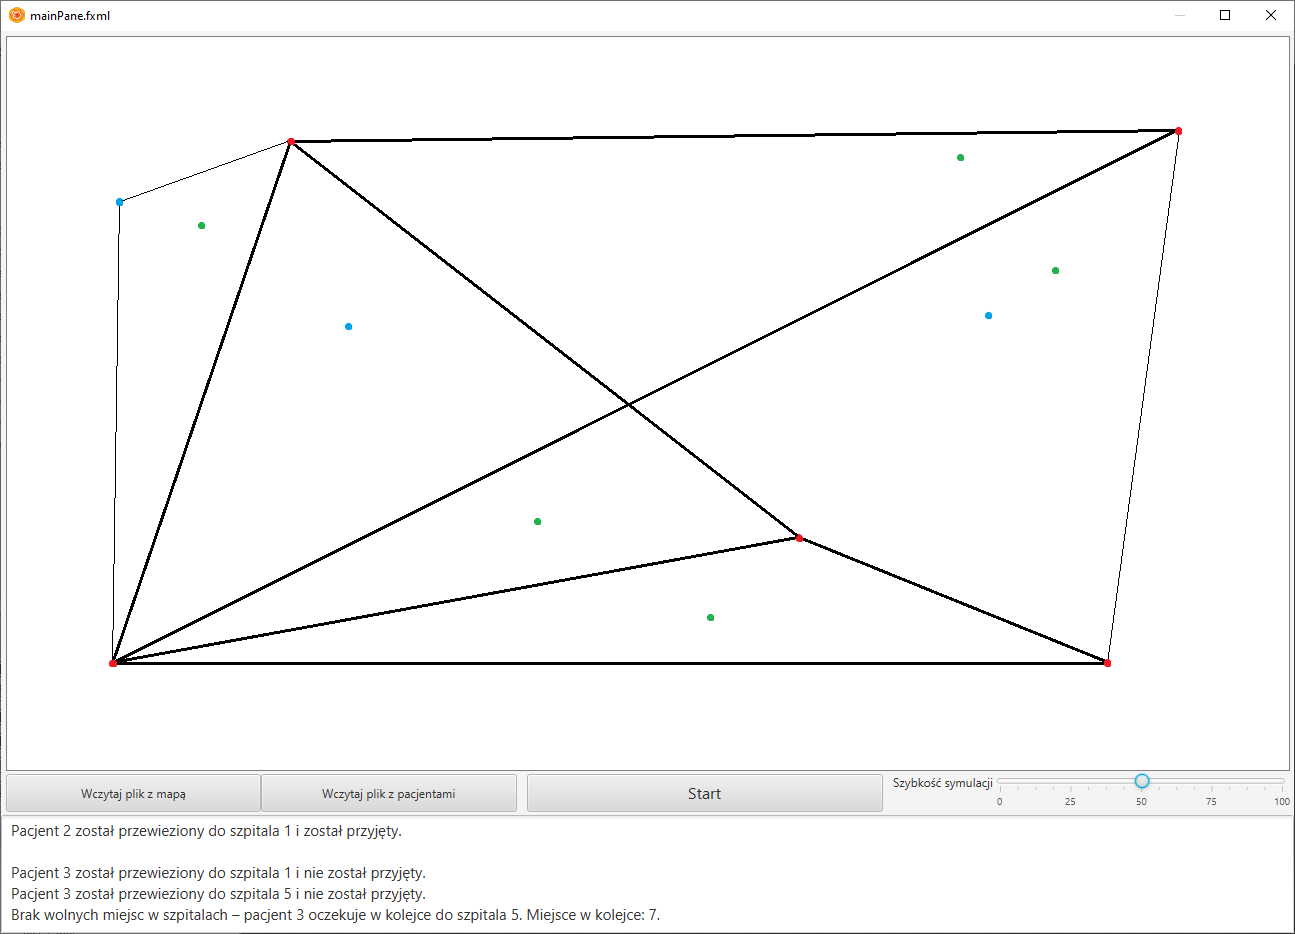
\includegraphics[scale=0.4]{gui.png}
    \end{center}
    Za wizualizację mapy (utworzenie planszy) będzie odpowiadało prostokątne płótno położone w górnej części okna. Pogrubione, czarne linie będą wizualizować drogi \textbf{pomiędzy szpitalami}, a cienkie, czarne linie \textbf{granice państwa} (najmniejszy zbiór wypukły zawierający w sobie wszystkie punkty). Szpitale, pacjenci oraz obiekty będą reprezentowane przez punkty o trzech możliwych \textbf{kolorach}:
    \begin{enumerate}
      \item Czerwony - szpital;
      \item Zielony - pacjent;
      \item Niebieski - obiekt.
    \end{enumerate}
    Użytkownik  będzie mógł dodać nowego pacjenta w miejscu, gdzie kliknął lewym przyciskiem myszy na plansze. \\
    Użytkownik za pomocą przycisków będzie mógł:
    \begin{enumerate}
      \item Rozpocząć/zatrzymać działanie symulacji (przycisk o dwóch możliwych nazwach ``Start'' lub ``Stop''. Nazwa
      zależy od tego, czy symulacja jest w trakcie działania);
      \item Wczytać plik, w którym znajdują się informacje o szpitalach, obiektach oraz drogach (przycisk ``Wczytaj plik z mapą'');
      \item Wczytać plik, w którym znajdują się informacje o pacjentach (przycisk ``Wczytaj plik z pacjentami'').
    \end{enumerate}
    Przy kliknięciu przycisku wczytującego plik z mapą lub plik z pacjentami użytkownikowi pojawi się dodatkowe okno, w którym będzie mógł wprowadzić nazwę pliku oraz przyciskiem ``Wczytaj'' wczytać plik o podanej nazwie do programu.

    \begin{center}
        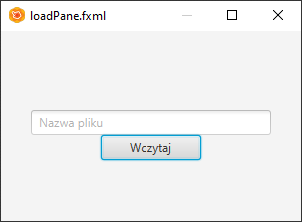
\includegraphics{okno.png}
    \end{center}

    Do sterowania szybkością przeprowadzanej symulacji służy suwak znajdujący się obok etykiety ``Szybkość symulacji''. Domyślna wartość tego suwaka to 50.

    Ustawienie suwaka będzie wpływało na \textbf{szybkość wyświetlanych komunikatów} w polu tekstowym znajdującym się na dole okna. Komunikaty będą informowały o tym, który pacjent został przewieziony do którego szpitala i czy został do tego szpitala przyjęty. Jeśli pacjent nie został przyjęty w żadnym szpitalu, to w polu tekstowym pojawi się informacja \textbf{o braku wolnych miejsc} w szpitalach oraz zostanie wypisane miejsce pacjenta w kolejce do szpitala, który był ostatnim szpitalem, w którym zatrzymał się pacjent.

    Pole tekstowe będzie również służyło do \textbf{wypisywania potencjalnych błędów} zawartych w plikach wejściowych oraz w sytuacji, gdy użytkownik będzie chciał dodać nowego pacjenta poza wyznaczonymi granicami.



\section{Testowanie}
    Główne \textbf{metody klas odpowiadających za operacje na danych} z pliku wejściowego będą testowane z wykorzystaniem biblioteki JUnit 4.12. Graficzny interfejs użytkownika będzie \textbf{testowany ręcznie} w trakcie implementacji oraz po zakończeniu pisania całości programu.

    Testowanie zostanie przeprowadzone na głównych metodach klasy odpowiedzialnej za \textbf{sterowanie symulacją} transportowania pacjentów do szpitali oraz głównych metodach klasy odpowiadającej za \textbf{operacje na danych z pliku wejściowego}. Metody zostaną przetestowane z poprawnymi oraz błędnymi danymi wejściowymi. Sprawdzone zostanie także działanie programu dla danych wejściowych będącymi \textbf{warunkami brzegowymi}.

\end{document}